\documentclass[compress,usepdftitle=false]{beamer}

\input{formatEPISENDiaporama}

\begin{document}

%***************************** Titre *******************************************
\begin{frame}
  \titlepage
\end{frame}

\begin{frame}
\ifthenelse{\equal{\TheLanguage}{french}}
 {\frametitle{Plan de la présentation}}
 {\frametitle{Presentation Outline}}
\tableofcontents
\end{frame}

%************************** Introduction **************************************
% \section[Introduction]{Introduction}
% % SLIDE
\begin{frame}
	\frametitle{Context}
	\begin{itemize}
		\item Competitive FPS depend on technical fairness: same rules, same information, for all players
		\item High stakes: esports prize pools (\$75 million at the 2026 EWC), professional careers, ranked progression
		\item Cheating (aimbots, wallhacks) directly threatens this integrity
	\end{itemize}
\end{frame}

% SLIDE
\begin{frame}
	\frametitle{The industry's answer, and its cost}
	\begin{itemize}
		\item Publishers responded with kernel-level (Ring 0) anti-cheat: full system visibility to catch cheats
		\item But: this grants a third-party driver unrestricted access to the entire machine, not just the game
		\item Raises real cybersecurity and privacy concerns
	\end{itemize}
	% \begin{center}
	% 	\hspace{-10mm}
	%   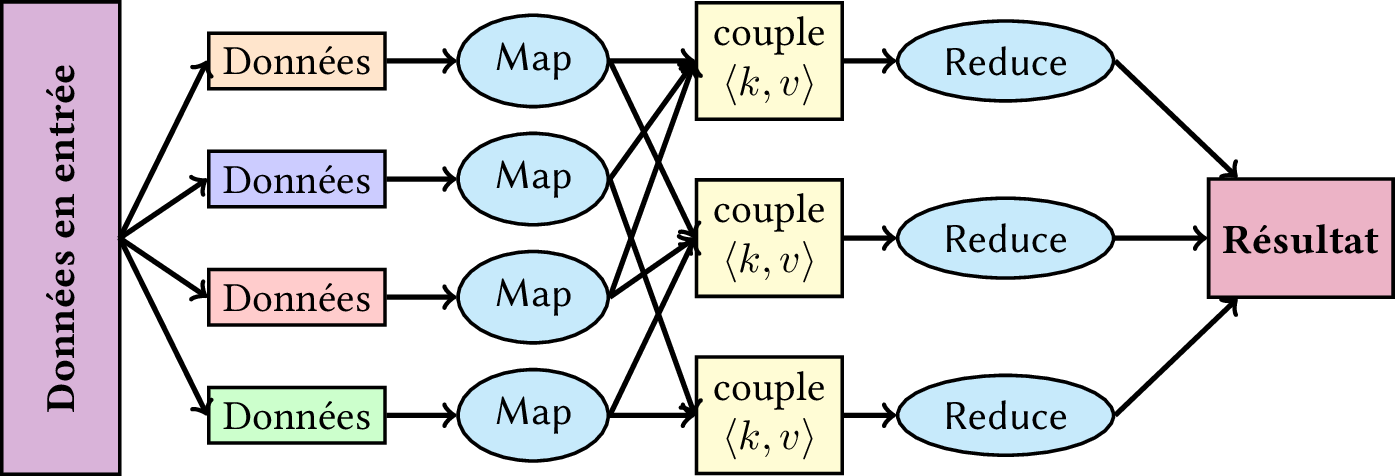
\includegraphics[height=2.7cm]{../images/Mapreduce.png}
	% 	\vspace*{-3mm}
	% \end{center}
\end{frame}

% SLIDE
\begin{frame}
	\frametitle{Problem}
	\begin{center}
		How can we detect cheating effectively without compromising system security through kernel-level access?
	\end{center}
\end{frame}


%************************** Ajout automatique des plans *****************************
\AtBeginSection[]
{
  \begin{frame}<beamer>
    \ifthenelse{\equal{\TheLanguage}{french}}
 		{\frametitle{Plan}}
 		{\frametitle{Outline}}
    \tableofcontents[currentsection,currentsubsection]
  \end{frame}
  \subsection*{$\empty$} % bidon, pour corriger un bug sur les sous-sections
}

%************************** Part one *******************************************
\section[Context and Problem]{Context and Problem}
% SLIDE
\begin{frame}
	\frametitle{Context}
	\begin{itemize}
		\item Competitive FPS integrity: same rules, same information, for everyone
		\item High stakes: \$75M prize pool at EWC 2026 (Paris), professional careers, ranked progression
		\item Cheats (aimbots, wallhacks) break this fairness
	\end{itemize}
\end{frame}

% SLIDE
\begin{frame}
	\frametitle{The industry's answer, and its cost}
	\begin{itemize}
		\item Anti-cheat moves to Ring 0: full visibility over memory and processes
		\item Cost: a third-party driver gets unrestricted access to the entire machine
		\item Risks: cybersecurity, system stability, user privacy
	\end{itemize}
	\begin{center}
		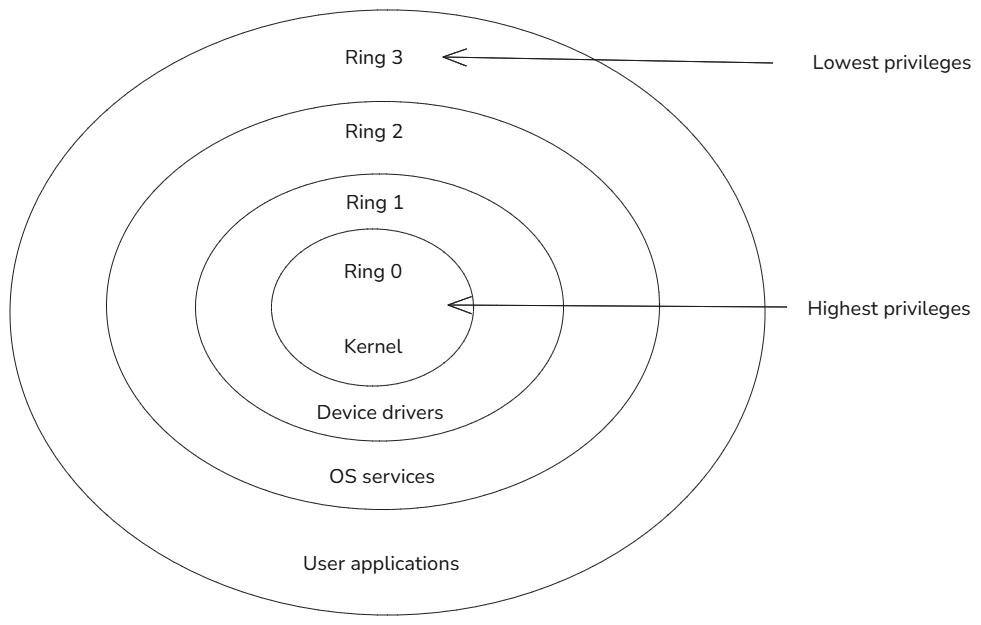
\includegraphics[height=4cm]{../images/chap01/fig4.png}
	\end{center}
\end{frame}

% SLIDE
\begin{frame}
	\frametitle{Problem}
	\begin{center}
		How can we detect cheating effectively without compromising system security through kernel-level access?
	\end{center}
\end{frame}


%************************** Part two *******************************************
\section[Structural Limits of Kernel-Level Anti-Cheat]{Structural Limits of Kernel-Level Anti-Cheat}
% SLIDE
\begin{frame}
	\frametitle{The arms race}
	\begin{itemize}
		\item Ring 0 anti-cheat forces cheat developers to match that privilege level: does not solve the problem, only moves it
		\item BYOVD: exploiting legitimate signed drivers to inject malicious code
		\item Asymmetry: anti-cheat needs rigorous validation to ship, evasion techniques ship in days
		\item[$\Rightarrow$] A race the defender cannot win
	\end{itemize}
\end{frame}

% SLIDE
\begin{frame}
	\frametitle{The hardware blind spot}
	\begin{itemize}
		\item DMA cheats: a PCIe card reads host RAM directly, at the hardware layer
		\item Processing offloaded to a second PC — nothing runs on the gaming machine
		\item No driver, no process, no software footprint $\Rightarrow$ invisible to Ring 0 anti-cheat
	\end{itemize}
	\begin{center}
		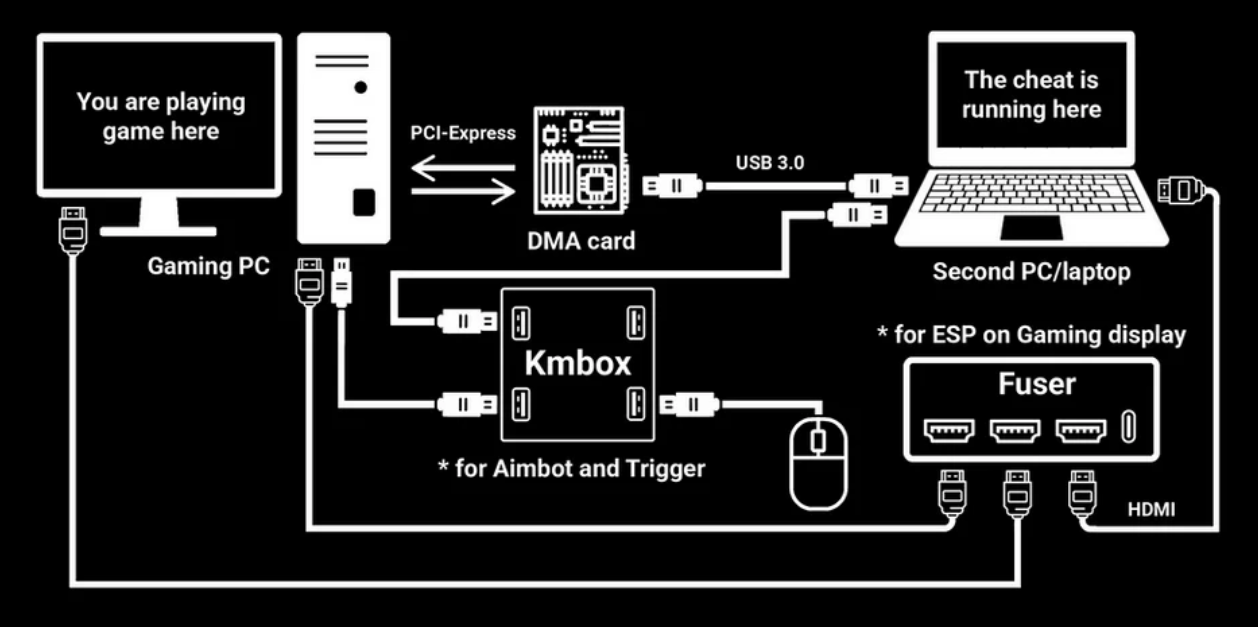
\includegraphics[height=4cm]{../images/chap01/fig5.png}
	\end{center}
\end{frame}

% SLIDE
\begin{frame}
	\frametitle{Experimental demonstration}
	\begin{itemize}
		\item Setup: isolated Windows 10 VM, Notepad seeded with a password, Windows-Kernel-Explorer + Cheat Engine
		\item Result: password located and reconstructed from RAM in minutes, with zero cooperation from the target process
		\item[$\Rightarrow$] Same inspection power a Ring 0 driver already has, by design, over every background process
	\end{itemize}
	\begin{center}
		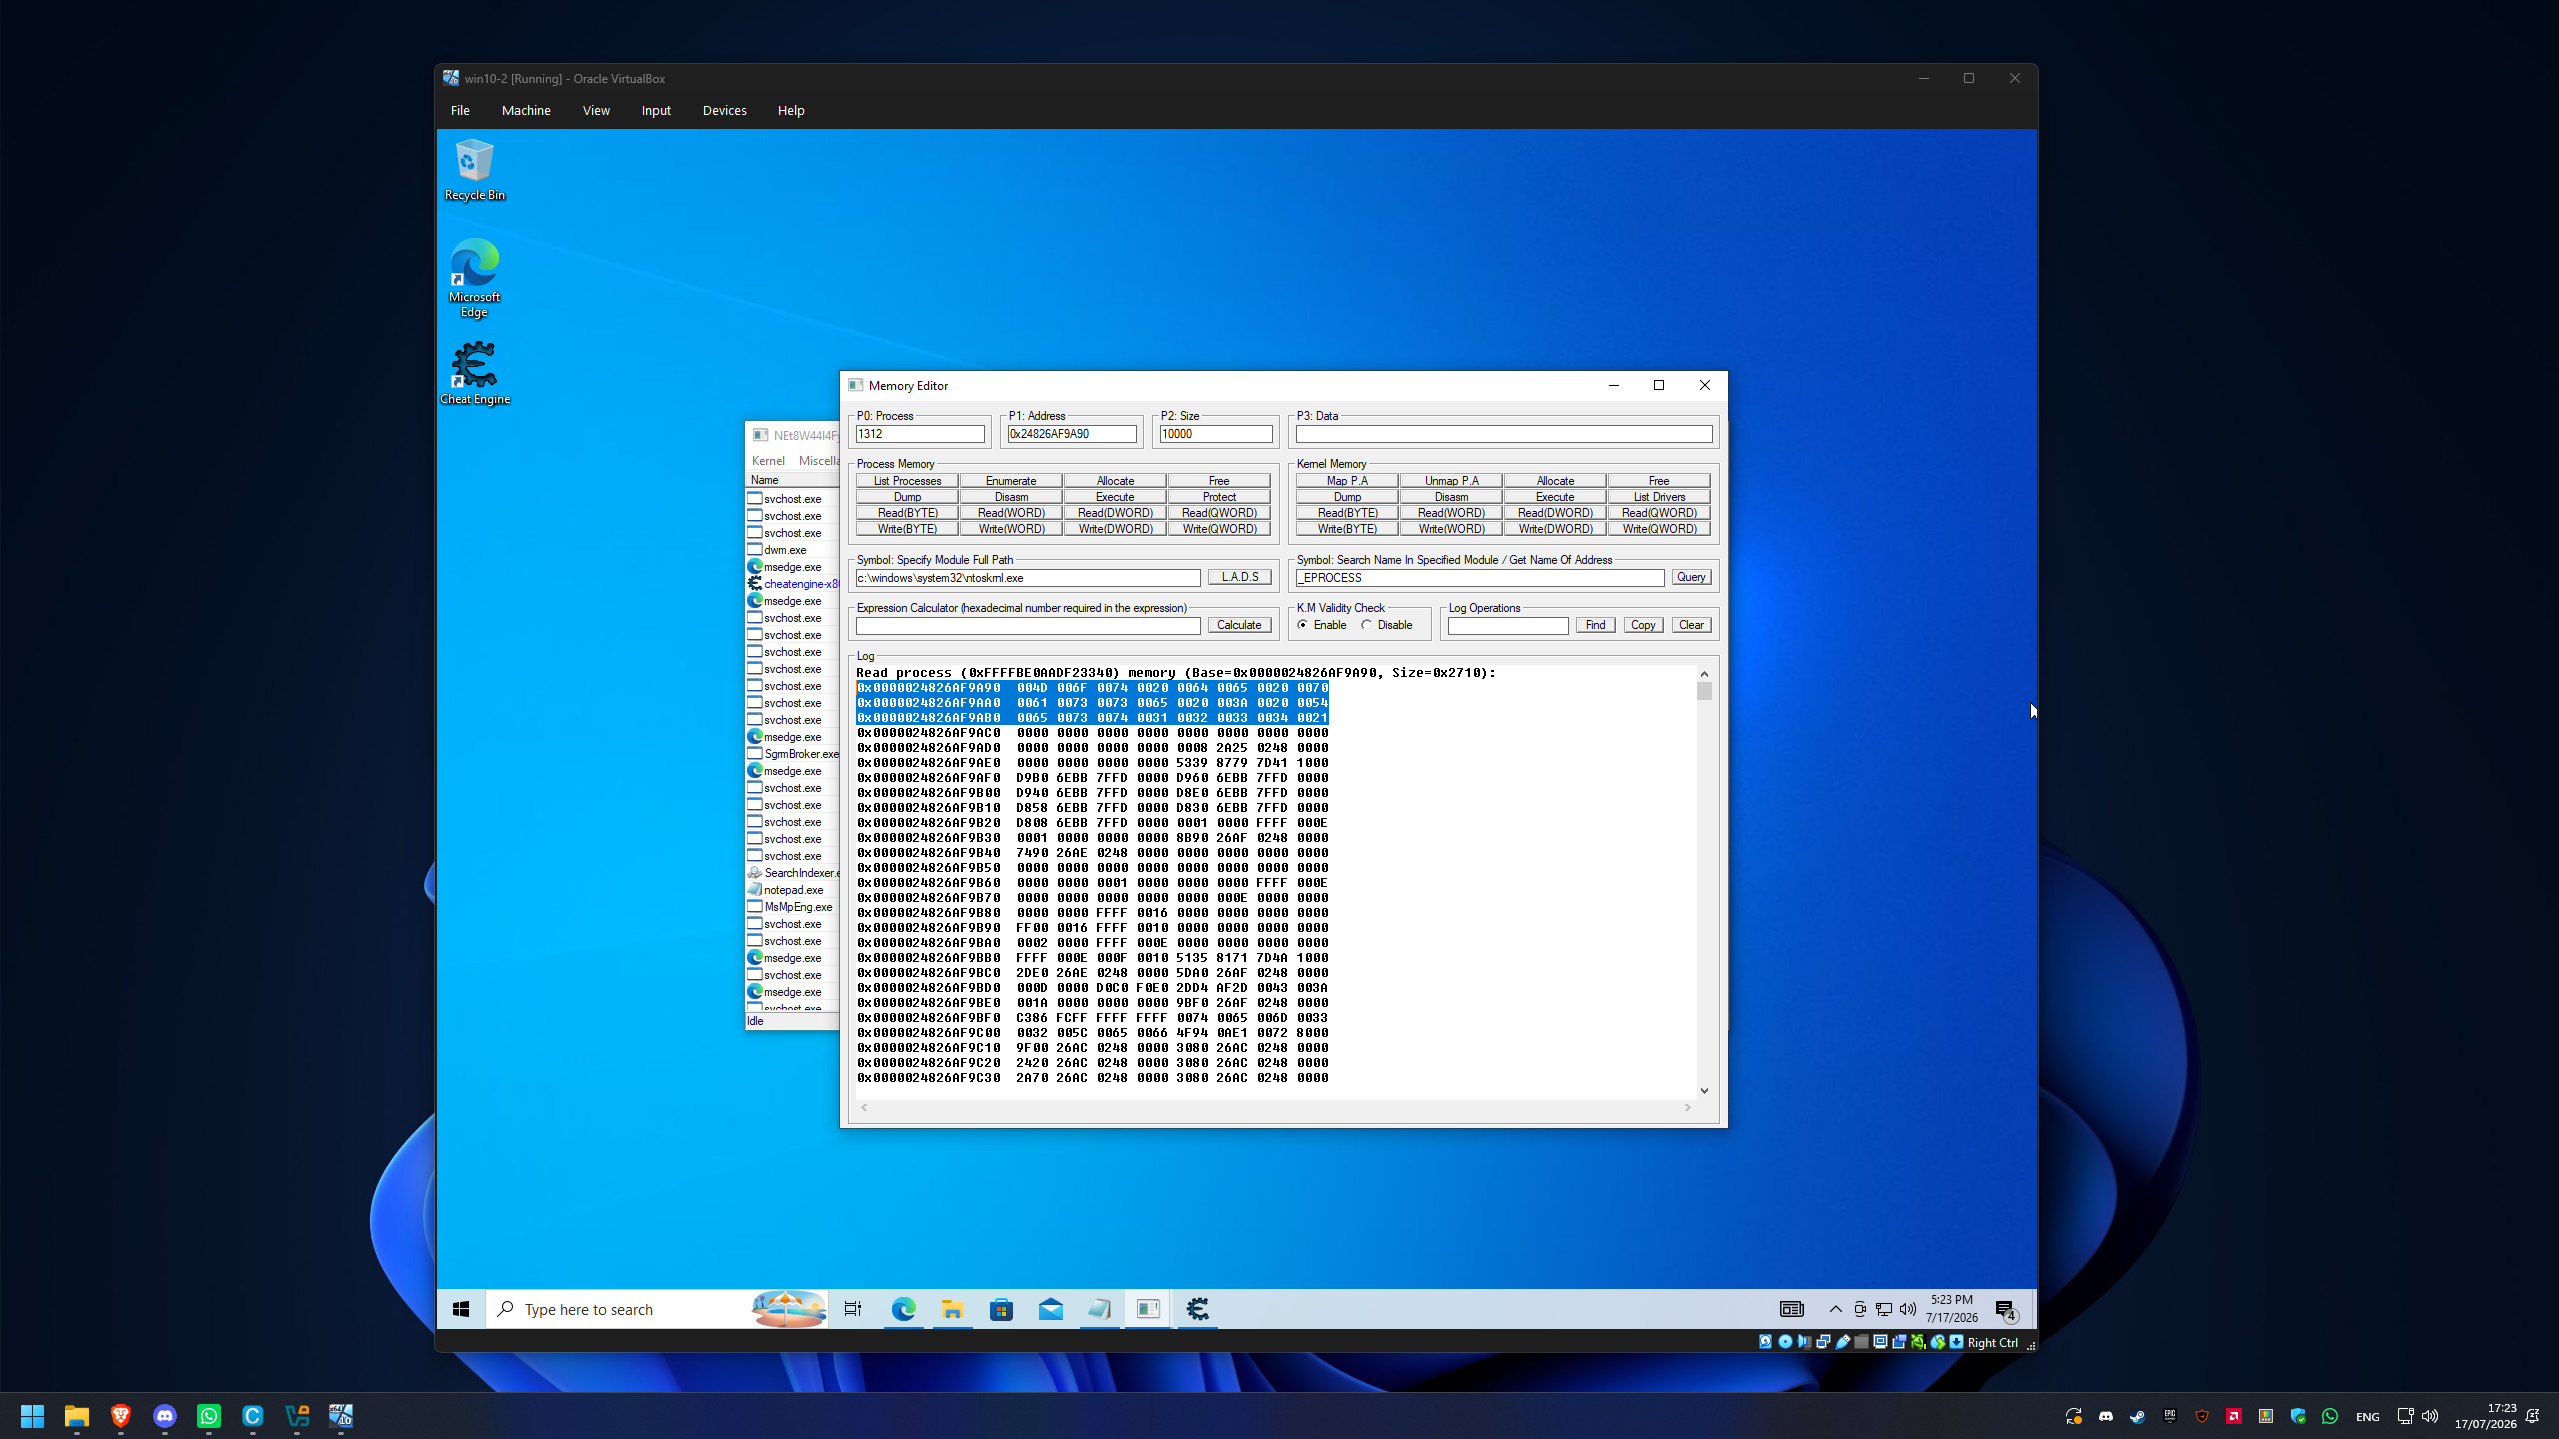
\includegraphics[height=4cm]{../images/chap02/15.png}
	\end{center}
\end{frame}

% SLIDE
\beamerdefaultoverlayspecification{}
\begin{frame}
	\frametitle{Problem}
	\visible<1->{
			If detection at this privilege level is both:
			\begin{itemize}
				\item Intrusive: capable of reading anything on the machine
				\item Bypassable: outpaced by DMA cheats
			\end{itemize}
		}
	\vspace{1cm}
	\visible<2->{
			\bf Is there a way to detect cheating without it?
		}
\end{frame}
\beamerdefaultoverlayspecification{<+->}


%************************** Part three *****************************************
\section[Server-Side Gameplay Analytics Pipeline]{Server-Side Gameplay Analytics Pipeline}
% SLIDE
\begin{frame}
	\frametitle{Shifting the trust anchor}
	\begin{itemize}
		\item Server is the authoritative source of match state: the client cannot tamper with it
		\item Analyze gameplay telemetry the server already receives, instead of inspecting the client
		\item No privileged access to the player's machine required
	\end{itemize}
\end{frame}

% SLIDE
\begin{frame}
	\frametitle{Pipeline architecture}
	\begin{itemize}
		\item Threshold scorer: 8 flags (time-to-damage, headshot ratio, reaction time, etc)
		\item LSTM scorer: tracks anomaly consistency across rounds and matches
		\item Suspicion score: weighted combination $\Rightarrow$ human review
	\end{itemize}
	\begin{center}
		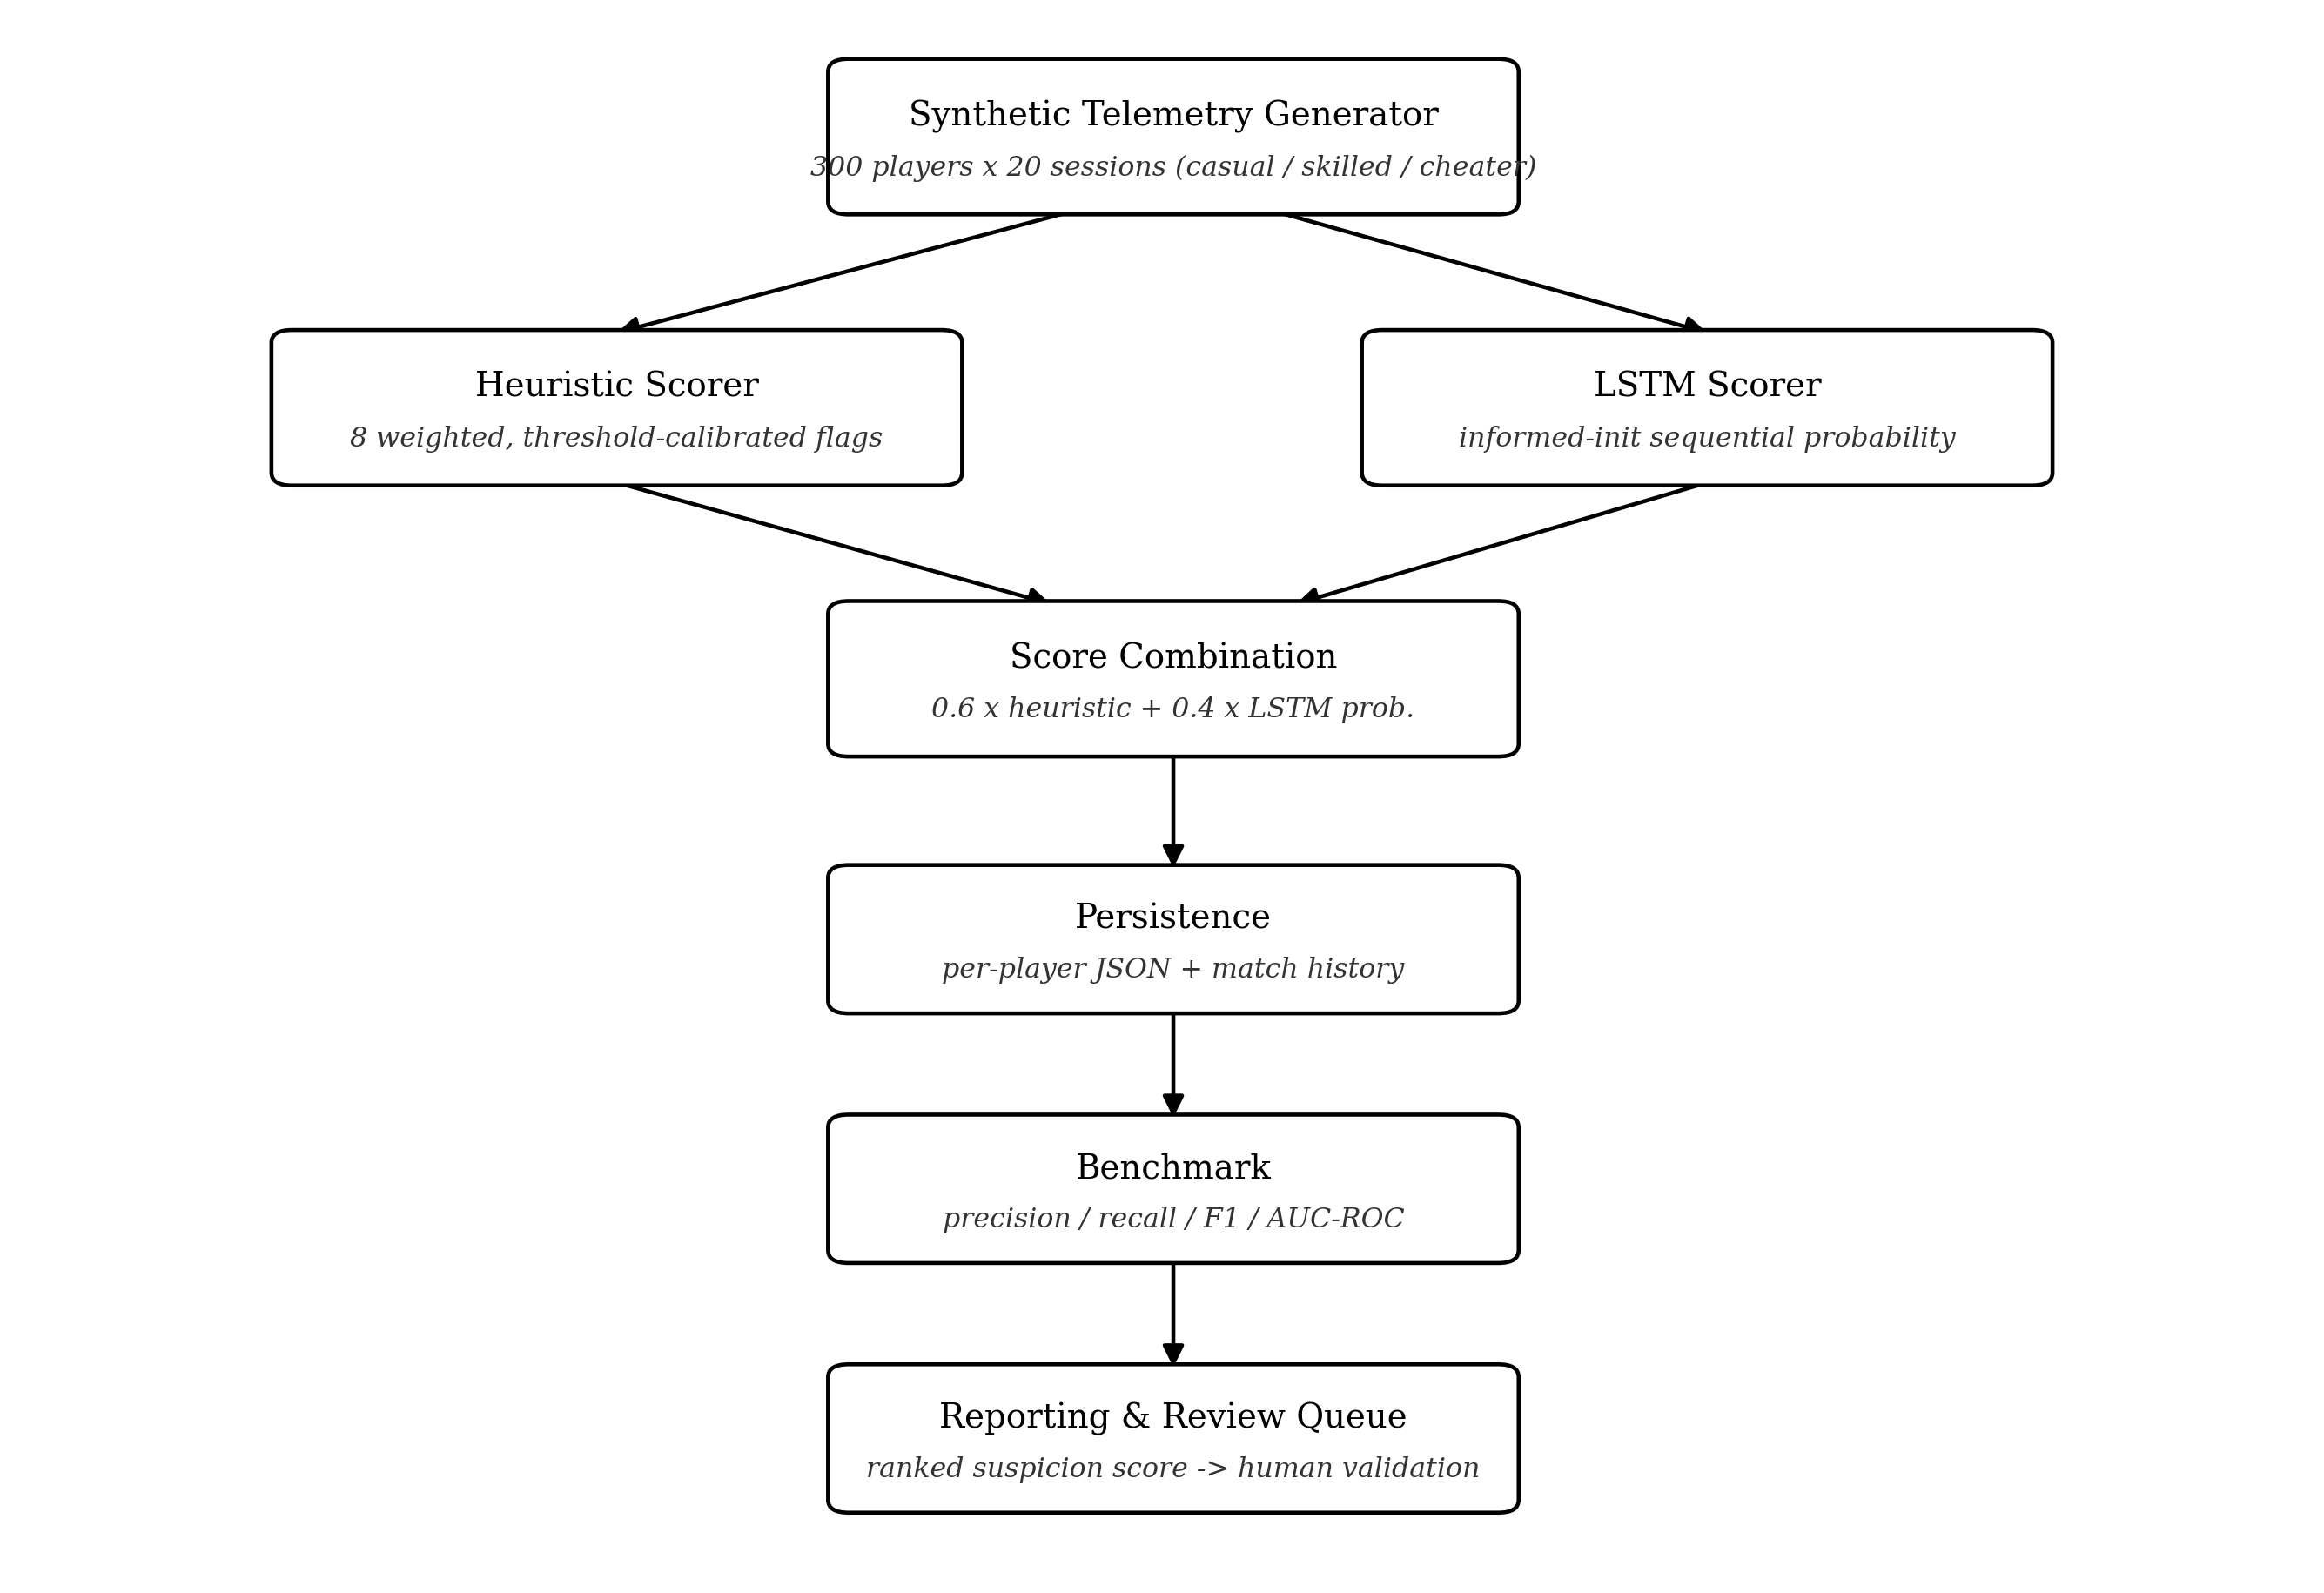
\includegraphics[height=4.5cm]{../images/chap03/pipeline_diagram.png}
	\end{center}
\end{frame}

% SLIDE
\begin{frame}
	\frametitle{Dataset design and the high-skill bias}
	\begin{itemize}
		\item Synthetic dataset: 300 players with casual / skilled / cheater profiles
		\item Calibrated from online benchmarks and personal experience
		\item Challenge: elite players can statistically resemble subtle cheaters
		\item Distributions deliberately overlapped around that boundary to empathize the hardest case
	\end{itemize}
	\begin{center}
		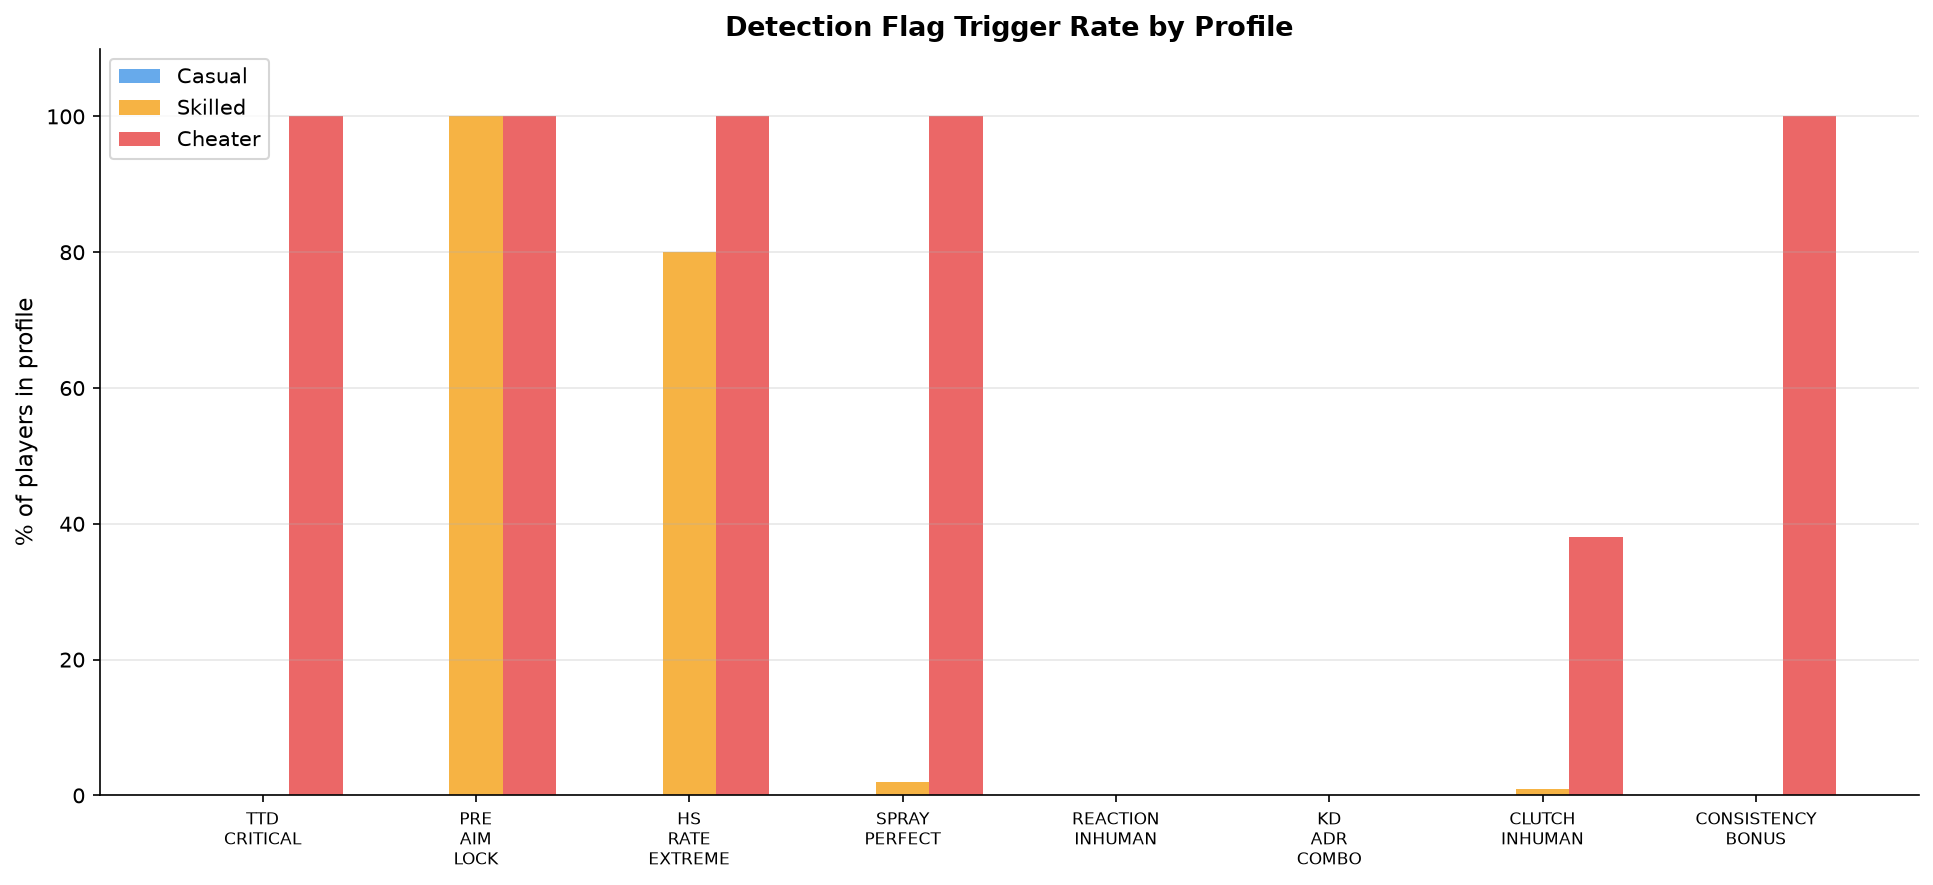
\includegraphics[height=3.5cm]{../images/chap03/flag_frequency.png}
	\end{center}
\end{frame}

% SLIDE
\begin{frame}
	\frametitle{Results}
	\begin{itemize}
		\item Clear statistical separation between legitimate players and cheaters at the population level
		\item \bf 0\% false positives on legitimate players, 51\% of cheaters correctly flagged
	\end{itemize}
	\begin{center}
		\begin{minipage}{0.48\textwidth}
			\centering
			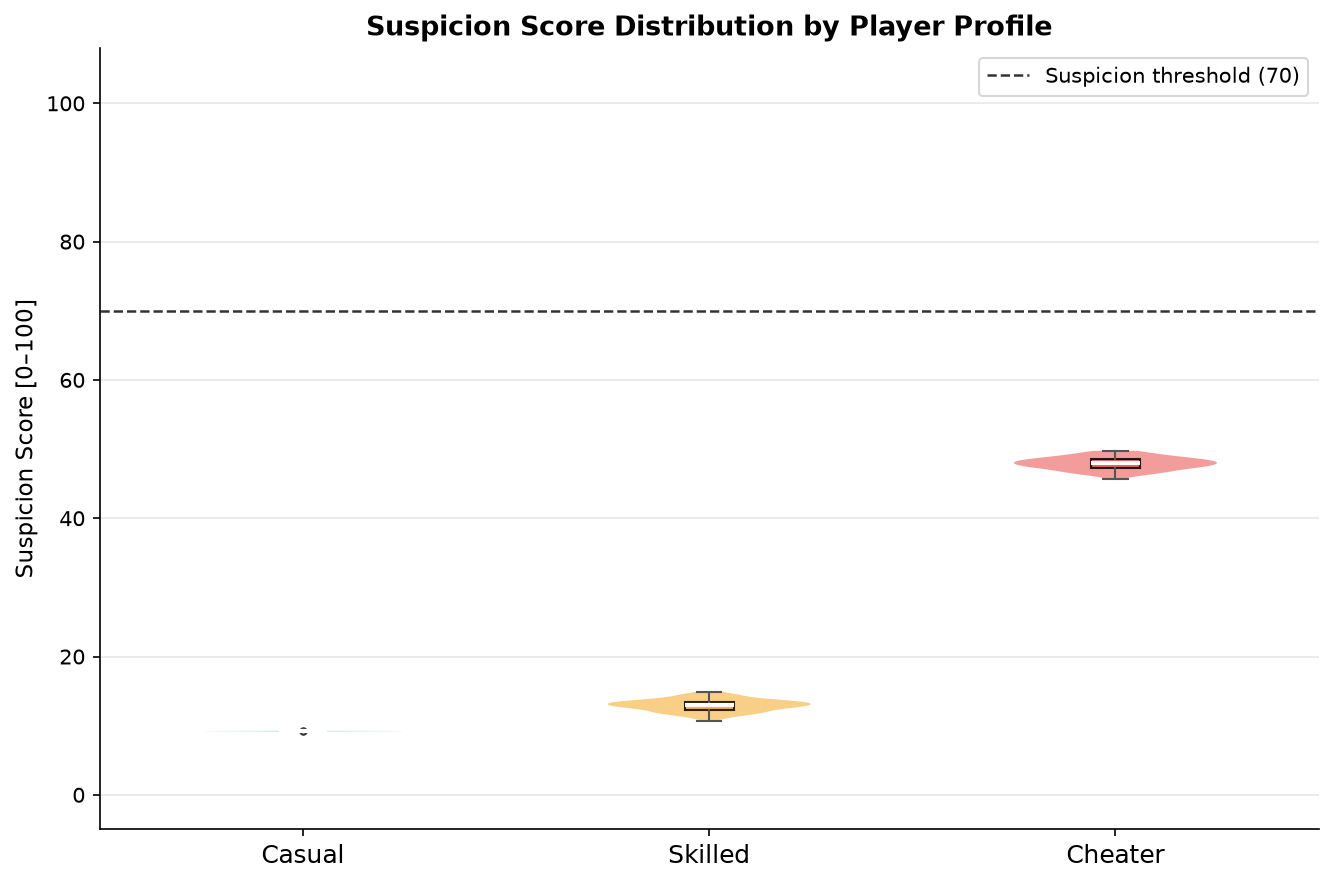
\includegraphics[height=3.75cm]{../images/chap03/score_distribution.png}
		\end{minipage}
		\hfill
		\begin{minipage}{0.48\textwidth}
			\centering
			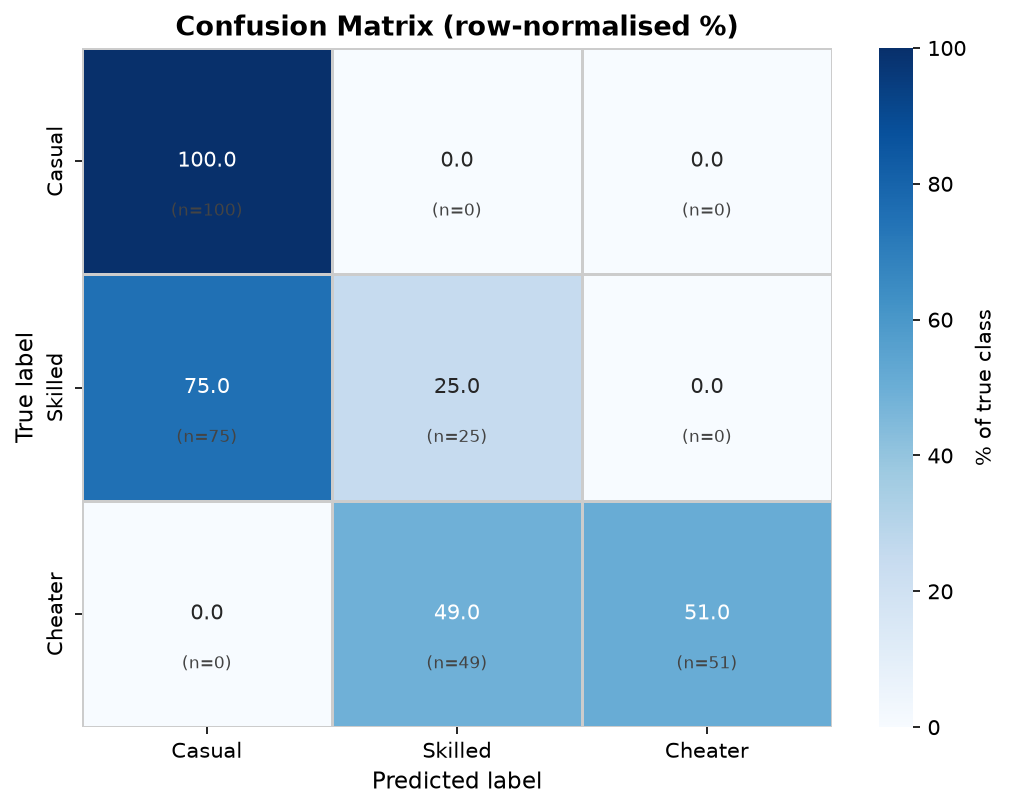
\includegraphics[height=3.75cm]{../images/chap03/confusion_matrix.png}
		\end{minipage}
	\end{center}
\end{frame}


%************************** Conclu ********************************************
\section[Conclusion]{Conclusion}
% SLIDE
\begin{frame}
	\frametitle{Limitations}
	\begin{itemize}
		\item Dataset and LSTM layer are entirely synthetic
		\item Flag thresholds are hardcoded instead of being trained
		\item Social features are not considered
	\end{itemize}
\end{frame}

% SLIDE
\begin{frame}
	\frametitle{Synthesis}
	\begin{itemize}
		\item Server-side behavioral analysis: viable, effective, privacy-preserving alternative to intrusive client drivers
		\item Removes the hardware blind spot created by DMA devices
		\item Ring 0 drivers cannot be the future of anti-cheat, given their privacy cost
		\item[$\Rightarrow$] Defense-in-depth: lightweight client checks + server-side scoring + human review
	\end{itemize}
\end{frame}

\plainframe{\Huge \begin{center} \color{redUPEC} Thank you for your attention! \\[1cm] Any questions?  \\ \end{center}}


\end{document}
